\documentclass{article}
\usepackage[a6paper,
            total={105mm, 148mm},
            margin=30pt,
            twoside % Tillåter olika placering av sidnummer på udda och jämna sidor
]{geometry}
\usepackage{fancyhdr}
\usepackage{parselines}
\usepackage{float}
\usepackage{graphicx}
\usepackage[absolute,overlay]{textpos}  % Package for absolute positioning
\usepackage{atbegshi}

\usepackage{imakeidx} % Registret
\usepackage{background} % Gråa Krusidull-E:et och alla bilder
\usepackage{ifoddpage} % Gråa Krudidull-E:et på udda sidor

% Normal background setup for odd pages
\backgroundsetup{
  scale=0.65,
  opacity=0.075,
  angle=0,
  color=black,
  vshift=-130,
  hshift=50,
  contents={%
    \checkoddpage
    \ifoddpage
      
\includegraphics[width=\paperwidth]{./bilder/large_E.png}
    \else
      %
\includegraphics[width=\paperwidth]{../bilder/VarumarkesBildServlet.jpg}
    \fi
  }
}


\newcommand{\custombackground}[1]{
  \backgroundsetup{
    scale=0.65,
    opacity=0.0,
    angle=0,
    color=black,
    vshift=-130,
    hshift=50,
    contents={\includegraphics[width=\paperwidth]{#1}}
  }
}

\newcommand{\noBackground}{
  \backgroundsetup{
    scale=0.65,
    opacity=0.0,
    angle=0,
    color=black,
    vshift=-130,
    hshift=50,
    contents={
\includegraphics[width=\paperwidth]{./bilder/no_background.png}}
  }
}


\newcommand{\resetBackground}{
  \backgroundsetup{
    scale=0.65,
    opacity=0.075,
    angle=0,
    color=black,
    vshift=-130,
    hshift=50,
    contents={%
      \checkoddpage
      \ifoddpage
        
\includegraphics[width=\paperwidth]{./bilder/large_E.png}
      \else
        %
\includegraphics[width=\paperwidth]{../bilder/VarumarkesBildServlet.jpg}
      \fi
    }
  }
}



% Disable indentation for the whole document
\setlength{\parindent}{0pt}


% Use fontspec with XeLaTeX or LuaLaTeX to load system fonts
\usepackage{fontspec}

% Set up the subsection font to Lucida Sans Unicode
\usepackage{titlesec}
\titleformat{\subsection}
  {\normalfont\fontsize{12pt}{10pt}\selectfont\fontspec{Lucida Sans Unicode}} % Adjust the size if needed
  {\thesubsection}{1em}{}

% Adjust vertical spacing around subsection titles
\titlespacing{\subsection}
{0pt}                % Left margin
{0.5ex plus .2ex}    % Space before subsection title (adjust as needed)
{0.5ex plus .2ex}    % Space after subsection title (adjust to decrease space after)

% Adjust footskip to add space below the footer
% \setlength{\footskip}{20pt} % Flyttar upp footern lite ########################################## Denna funkar inte riktigt som jag trodde. Jag vill flytta upp sidnumret lite mer
\setlength{\textheight}{120mm}


% Define the page style
\fancypagestyle{main}{
  \fancyhf{} % clear all header and footer fields
  \fancyhead[RO]{\hfill \footnotesize\scshape\leftmark \hfill}
  % \fancyfoot[LE,RO]{\thepage}

  % Adjust the page number position
  % Set page number closer to the edge by increasing the right margin
  \fancyfoot[LE]{\hspace{-17pt}\thepage} % Flytta ut sidnummer jämna sidor
  \fancyfoot[RO]{\thepage\hspace{-17pt}} % Flytta ut sidnummer udda sidor

  % Ta bort linje under/över header och footer
  \renewcommand{\headrulewidth}{0 pt}
  \renewcommand{\footrulewidth}{0 pt}

  % Använder footnote for 'visste du att'
  \renewcommand{\footnoterule}{}
  \renewcommand{\thefootnote}{}
}

% Set up textblock package to work with A6 paper
\setlength{\TPHorizModule}{1mm}  % Set horizontal units to mm
\setlength{\TPVertModule}{1mm}   % Set vertical units to mm

% Define the custom command to place text at the bottom of the page
\newcommand{\vissteduatt}[1]{%
    \begin{textblock*}{100mm}(12mm,137mm) % Adjust (2.5mm, 140mm) to position text
        \raggedright
        {\footnotesize{\textit{#1}}}
    \end{textblock*}
    \newpage % Ensures that the text appears only on the current page
}


% Define the custom command for small font and italics
\newcommand{\songinfo}[1]{%
  \textit{\small #1 \\}%
}









% DETTA SÄTTET ATT GÖRA REGISTER FUNGERAR BRA OCH ÄR LÄTT MEN DET BLIR INTE LIKA SNYGGT UTAN PUNKTERNA



% HITTA ETT SÄTT ATT GÖRA ETT SNYGGARE REGISTER INNAN VI FORTSÄTTER ATT LÄGGA TILL LÅTAR ETC. 
\makeindex[ % Alfabetiskt register
  name=alfa,
  columns=1,
  title=Alfabetiskt Register,
  intoc,
  options = {-s styleAlfa.ist}
]
\makeindex[ % Analfabetiskt register -- början av sången
  name=anfa,
  columns=1,
  title=Analfabetiskt Register,
  intoc,
  options = {-s styleAlfa.ist}
]


\begin{document}

% Apply the 'main' page style
\pagestyle{main}

% Title and empty page without header/footer
\NoBgThispage
\begin{titlepage}
    \centering
    \vspace{1cm}
    {\fontsize{18}{18}\selectfont E-sektionens sångbok}\\
    \vspace{0.2cm}
    {\fontsize{30}{30}\textbf{Komponenten}}\\
    \vspace{0.2cm}
    {\fontsize{15}{15}\textit{2:a upplagan}}
    \thispagestyle{empty}

    \begin{figure}[H]
      \centering
      
\includegraphics[width=1\textwidth]{./bilder/large_E.png}
    \end{figure}

\end{titlepage}


\newpage


Borra ett hål i pärmen här för att fästa din penna: {\Huge $\bullet$}

\subsubsection*{Konsten att sjunga!}
Att sjunga är verkligen något av det roligaste som finns\dots


Jag vet inte riktigt vad vi vill skriva här\dots

Att sjunga är kul\dots



Morris Thånell BME19 och Elin Helmersson E21\\
Sångbokskommittén 2024



\newpage

Tack till de som hjälpt oss med boken!

\newpage

\begin{center}
    \textbf{Viktig information}
\end{center}

% \backgroundsetup{ 
%   scale=0.36,
%   opacity=1,
%   angle=0,
%   color=black,
%   vshift=300,
%   hshift=151,
%   contents={
\includegraphics[width=\paperwidth]{./bilder/profilbild.png}}
% }

\begin{textblock*}{6cm}(6cm,1.5cm) % {block width}(x-coordinate, y-coordinate)
  
\includegraphics[width=3.5cm]{./bilder/profilbild_stor.png} % Adjust the image size as needed
\end{textblock*}
\begin{parse lines}[\noindent]{#1\\}
    Ägare:

    Sektion(?):
    
    Inskrivningsår:
    
    Födelsedatum:



    Lämna tillbaka mig till den här adressen:


    Hittelön:
    Om jag inte varit teknolog hade jag varit:
    Om jag fick välja nollningstema:


    Favoritmat:
    Favoritband:
    Favorit
    Bästa 
    Favoritintegral:
    
    .... Rita eller klistra en bild

\end{parse lines}

\newpage

% \subsubsection*{Innehållsförteckning}
\tableofcontents

\newpage
\begin{center}
  \vspace*{1.5cm}
  {\fontsize{20}{20}\textbf{Vett och etikett}}\\
  \vspace{0.7cm}
  {\fontsize{12}{12}\textit{Om den pryde själv får välja}}
\end{center}
\addtocwithheader{Vett och etikett}  % Add entry to TOC and set header
\noBackground
\newpage

\subsubsection*{KLÄDKOD}
För att underlätta förmedlingen av vem som ska ha på sig vad använder vi oss av följande namn.

\textbf{Truls}: Manlig teknolog\\
\textbf{Trula}: Kvinnlig teknolog\\
\textbf{Trelsa}: För hen som inte vill identifiera sig med någon av ovanstående.\\

\subsubsection*{Högtidsdräkt - Militäruniform och folkdräkt}

\textbf{Truls}: Militäruniform, folkdräkt eller frack\\
\textbf{Trula}: Militäruniform, folkdräkt eller balklädding\\
\textbf{Trelsa}: Se Truls/Trula\\

\subsubsection*{Civil högtidsdräkt}

\textbf{Truls}: Frack, vit skjorta, vit fluga\\
\textbf{Trula}: Balklädding\\
\textbf{Trelsa}: Se Truls/Trula\\

\subsubsection*{Smoking}
\textbf{Truls}: Smoking, vit skjorta, svart fluga\\
\textbf{Trula}: Lång klänning, dock behöver den inte vara lika elegant som en Balklädding. Tänk festligt.
\textbf{Trelsa}: Se Truls/Trula\\

\subsubsection*{Mörk kostym}
\textbf{Truls}: Mörkblå, mörkgrå eller svart kostym. Vit skjorta med sidenslips eller fluga i valfri färg.\\
\textbf{Trula}: En finare känning, men även byxdress elelr halvlång kjol med jacka går bra.\\
\textbf{Trelsa}: Se Truls/Trula\\

\subsubsection*{Kavaj}
Ibland även kallad bruten elelr udda kavaj.\\
\textbf{Truls}: Kavaj och ett par finare byxor (dock inte kostymbyxor), skjorta i valfri färg. Fluga eller slips kan vara trevligt!\\
\textbf{Trula}: Cocktailklänning, kjol eller dress.\\
\textbf{Trelsa}: Se Truls/Trula\\

\subsubsection*{Mörk kostym}
\textbf{Truls}: Ouvve \textbf{Hur vill vi stava ouvve/ovve i boken?}\\
\textbf{Trula}: Ouvve\\
\textbf{Trelsa}: Se Truls/Trula\\


\subsubsection*{KLÄDKOD version 2?}
Kåren har ett annat upplägg på hur de visar klädkoderna. Vill vi göra som dem?
\\

Exempel (kopierat från kårens bok)

\subsubsection*{Högtidsdräkt/högtidsklädsel}
För honom är frack lämplig. 
En fin golvlång klänning gäller för henne 
- ett bra material och ett tjusigt sntit ska det vara på den. 
Vill man bära handskar till klänningen går det bra, 
men glöm inte att ta av dem när du äter. 
Både han och hon kan istälet bära hembygdsdräkt eller militär högtidsdräkt.


\newpage

\subsubsection*{ETIKETT}

\subsubsection*{Vid bordet}
Han har sin bordsdam till höger om sig och hon har sin bordsherre till vänster.
Herren drar ut stolen till höger för att hjälpa sin bordsdam till bords eller från bordet. 


\textbf{Denna visste du att måste nog skrivas om eller ändra storleken på all text i boken. Vi ahr lite större text än i gamla komponenten vilket göra att vi inte får plats med riktigt lika mycket text på varje sida....}

\vissteduatt{Visste du att bordsherre och bordsdam är bordsplaceringsbenämningar\\ som avser att underlätta sittningsförfarande och är helt könsneutralt?}

\input{kapitel/01-sånger.tex}

\begin{center}
    \vspace*{1.5cm}
    {\fontsize{20}{20}\textbf{E-sektionens visor}}\\
    \vspace{0.7cm}
    {\fontsize{12}{12}\textit{Om E:aren själv får välja}}  
\end{center}
\addtocwithheader{E-sektionens visor}  % Add entry to TOC and set header
\noBackground

\newpage
\resetBackground


\subsection*{E-sektionens Kampvisa I}
\index[alfa]{E-sektionens Kampvisa I}
\index[anfa]{Det sprakar så glatt i vårt hår}
\songinfo{Mel: Stars and Stripe \textbf{OSÄKER MELODI?}}

\begin{parse lines}[\noindent]{#1\\}
    Det sprakar så glatt i vårt hår
    ur öronen sprutar det gnistor
    och strömmarna i våra tår
    laddar upp oss när vi går.

    I hjärnan vi har resistans
    och ström genom motstånd ger en spänning
    och spänning det vill vi ju ha.
    Vi går på E! Vi går på E!
    Vi går på Elström!

\end{parse lines}


\subsection*{E-sektionens Kampvisa II} 
\index[alfa]{E-sektionens Kampvisa II}
\index[anfa]{E, E, E vill vi se}
\songinfo{Mel: Trink, trink, brüderlein trink}

\begin{parse lines}[\noindent]{#1\\}
    E, E, E vill vi se
    E är det bästa där é
    E, E, E vill vi se
    E får oss alla att le!
    Spänning där é i vär erotik
    vi kör med medicin och teknik.
    Spänning där é i vår erotik
    vi kör med elektroteknik

\end{parse lines}

\vissteduatt{Visste du att E-sektionen har sjukt många kampvisor? ELLER \\Visste dua tt Kampvisa II reviderades för att innefatta båda utbildningarna på E-sektionen?}

% \newpage

\subsection*{E-sektionens Kampvisa III} 
\index[alfa]{E-sektionens Kampvisa III}
\index[anfa]{Vi é elteknister ifrån LTH}
\songinfo{Mel: Vi äro musikanter}

\begin{parse lines}[\noindent]{#1\\}
    Vi é elteknister ifrån LTH.
    Hos oss finns inga brister och dé é ju som så.

    (Att) Vi kan lödda, räkna, dricka, bränna sprit.
    Upp till Lophtet, kom så går vi dit!

    Vi kan räkna tangens, sinus, derivera, integraler.
    Vi kan koda singelchip och mata våran pic.

    Ett in, noll ut, rulla kabel, heja vit!
    Vi vill att just du skall komma hit.

    Hoppa i din vita overall och börja gå.
    Elteknik på LTH det bästa du kan få!

\end{parse lines}


\subsection*{E-sektionens Kampvisa IV} 
\index[alfa]{E-sektionens Kampvisa IV}
\index[anfa]{Vi vill ha mera E}
\songinfo{Mel: Mera mål}

\begin{parse lines}[\noindent]{#1\\}
    Vi vill ha mera E, flera E
    Å E det kommer ni att se
    Vi vill ha mera E, mycket mer
    Se upp här kommer vi från E

\end{parse lines}

\vissteduatt{Visste du att E-sektionen är den äldsta sektionen på LTH?}

\newpage


\subsection*{E-sektionens Kampvisa V} 
\index[alfa]{E-sektionens Kampvisa V}
\index[anfa]{Alla vi på E-sek klappar nu} % VILL VI HA DENNA ENS?
\songinfo{Mel: Klappa händerna}

\begin{parse lines}[\noindent]{#1\\}
    //: Alla vi som går på E-sek klappar nu ://

\end{parse lines}


\subsection*{E-sektionens Kampvisa VI} 
\index[alfa]{E-sektionens Kampvisa VI}
\index[anfa]{Vi går på E-sek}
\songinfo{Mel: Man ska ha husvagn}

\begin{parse lines}[\noindent]{#1\\}
    Vi går på E-sek, och vi har spänning så som få
    Vi går på E-sek, äldst och bäst på LTH
    Vi går på E-sek, vår färg är vit, Elektrovit!
    Vi går på E-sek, LTH:s elit!

\end{parse lines}


\begin{textblock*}{3cm}(3.5cm,8.9cm) % {width}(x, y)
    
\includegraphics[width=4.5cm]{./bilder/Transistorer.png}
\end{textblock*}

\vissteduatt{Visste du att några kampvisor blivit reviderade i efterhand?}


\newpage

\subsection*{E-sektionens Kampvisa VII} 
\index[alfa]{E-sektionens Kampvisa VII}
\index[anfa]{E-sek på LTH} 
\songinfo{Mel: Anton aus Tirol \\ Text: Sebastian Elm (E12), Kewin Erichsen (E11)}

\begin{parse lines}[\noindent]{#1\\}
    ||: E-sek, E-sek, E-sek på LTH :||
    Vi slajdar in,
    med grym entré
    För det är vi som går på E!
    Vi lyser upp med bra manér,
    tänder gnistan inom er
    Det är eliten som ni ser!

    Är du för klen?
    De' e ingen kris
    Det fixar vi med dialys!
    När ni sedan vaknat opp,
    är vår spänning än på topp
    För det är vi som går på E!
    ||: E-sek, E-sek, E-sek på LTH :||

\end{parse lines}

\subsection*{E-sektionens Kampvisa VIII} 
\index[alfa]{E-sektionens Kampvisa VIII}
\index[anfa]{Alla vill höra våran sång} 
\songinfo{Mel: Anton aus Tirol \\ Sebastian Elm E12 \& Kewin Erichsen E11}

\begin{parse lines}[\noindent]{#1\\}
    Alla vill höra våran sång
    Därför vi sjunga gång på gång
    E-sek, här kommer E-sek
    Och alla andra, de kommer igång

\end{parse lines}

\vissteduatt{Visste du att kampvisa VII har en musikvideo på Youtube?}

\newpage


\subsection*{E-sektionens Kampvisa IX} 
\index[alfa]{E-sektionens Kampvisa IX}
\index[anfa]{Här kommer E-sektionen} 
\songinfo{Mel: Gärdebylåten}

\begin{parse lines}[\noindent]{#1\\}
    Här kommer E-sektionen
    Vackrast på hela jorden
    Tuborg i Edekvata, billigast i hela Lund
    Med vitt ska vi kiosken måla
    Sen för vår seger skåla
    Festa det gör vi bäst på E
    O alla får va me’
    \textbf{(Om man vill, Och det vill man!)}

\end{parse lines}


\subsection*{E-sektionens Kampvisa X} 
\index[alfa]{E-sektionens Kampvisa X}
\index[anfa]{Everywhere we go} 
%\songinfo{Mel: Gärdebylåten}

\begin{parse lines}[\noindent]{#1\\}

    Everywhere we go! \textit{Everywhere we go!}
    People wanna know! \textit{ People wanna know!}
    Who we are! \textit{Who we are!}
    So we tell them! \textit{So we tell them!}
    We are the E-sek! \textit{We are the E-sek!}
    Mighty mighty E-sek! \textit{Mighty mighty E-sek!}

    Oh ah å E-sek...

\end{parse lines}
\vissteduatt{Visste du att E-sektionen äger rättigheterna till F:s F och hyr ut \\det för den administrativa kostnaden att upprätthålla rättigheten?}
\newpage


\subsection*{E-sektionens Kampvisa XI} 
% \index[alfa]{E-sektionens Kampvisa X}
% \index[anfa]{Everywhere we go} 
\songinfo{Mel: \\Text:}

\begin{parse lines}[\noindent]{#1\\}
    

\end{parse lines}


\vissteduatt{Visste du att här kan man fylla i nya kampvisor?}
\newpage

\subsection*{E-sektionens Sexlåt} 
\index[alfa]{E-sektionens Sexlåt}
\index[anfa]{Sexets låt} 
\songinfo{Mel: När vindarna viskar mitt namn\\
Text: Sebastian Elm E12, Kewin Erichsen E11
}

\begin{parse lines}[\noindent]{#1\\}
    Jag var fångad i sexet, jag såg inget ljus
    In i dimman betygen försvann
    Jag jobbar och sliter, det finns ingen tid
    När FAN låg jag senast i fas

    Men de ger mig min styrka, ger mig sprit att förtära var natt
    En fyllecell, vårt mål, vi trivs bäst i vår vita kavaj!

    Vi mår va några jävla drägg, som går loss och dricker rent
    Men E6 styr upp spänningen

    //: När Gasquen den viskar vårt namn ://

\end{parse lines}

\vissteduatt{Visste du att "Gasquen" kan bytas till aktuell plats där sången
\\ framförs?}

\newpage

\subsection*{Medtekingenjören} 
\index[alfa]{Medtekingenjören}
\index[anfa]{Vi som botar alla sjuka} 
\songinfo{Mel: O hur saligt att få vandra
}

\begin{parse lines}[\noindent]{#1\\}
    Vi som botar alla sjuka
    Diagnos med hjälp av ultraljud
    Hårda delar liksom mjuka
    Vi placerar elektroder på din hud
    Och studerar sen effekten
    Tolkar diagrammets amplitud
    Om den påvisar defekter
    Med din hjärna så leker vi gud

    //: En röntgenbild, den gör mig vild
    och jag blir kär, får hjärtbesvär
    En blå pastill, och lite pill
    Får mig att tända till ://

    Gener kan manipuleras
    Ingenjörskonst på ett högre plan
    När vi dig har programmerat
    Blir du aldrig mer likadan
    Läkarna behandlar dig mot gaser
    Rektoskopi ja det slipper vi
    Istället leker vi med laser
    Och röntgen och MRI

\end{parse lines}

\vissteduatt{Visste du att  denna låt är skriven av MiT på KTH?}

\newpage

\begin{parse lines}[\noindent]{#1\\}
    Och läkarsprit - vår favorit
    Ja läkarsprit - mot hepatit
    Sälj läkarsprit - ge oss profit
    Mer läkarsprit

    Mer läkarsprit - fyll på ge hit
    Jag får aptit - av läkarsprit
    För läkarsprit - vår favorit
    Mer läkarsprit

\end{parse lines}

\begin{textblock*}{3cm}(0.2cm,5.1cm) % {width}(x, y)
    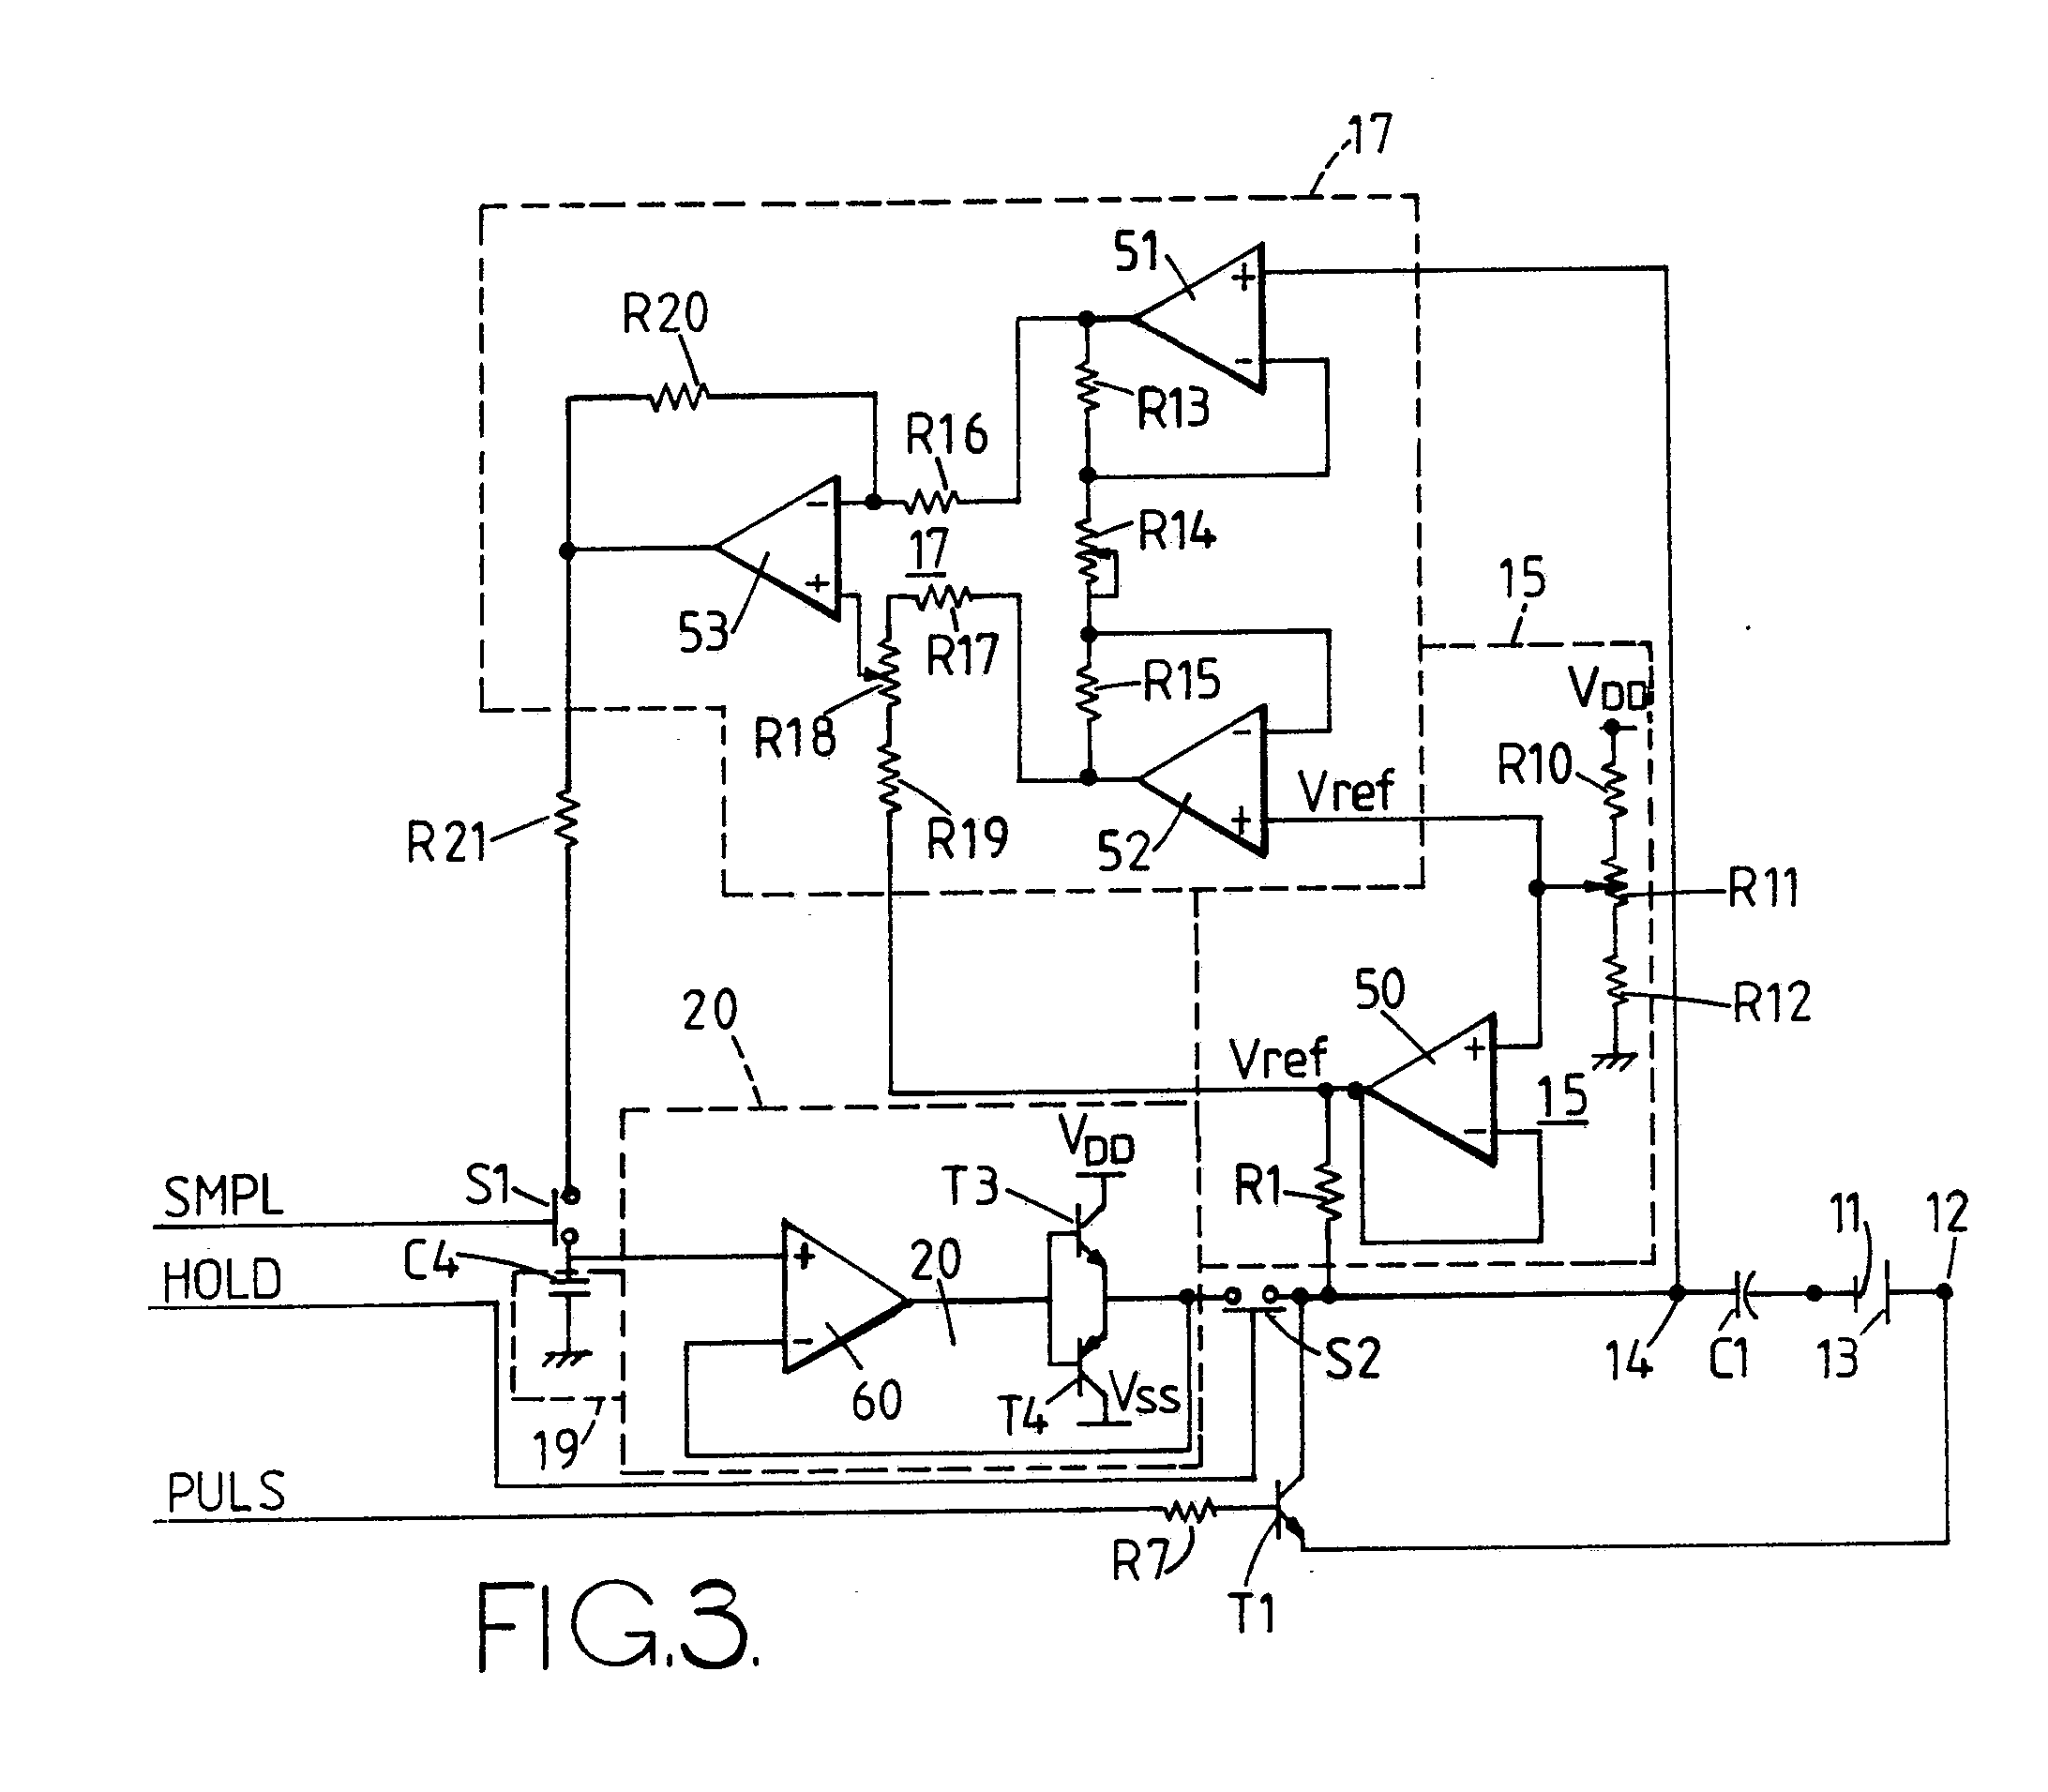
\includegraphics[width=9.9cm]{./bilder/PacemakerCircuit.png}
\end{textblock*}

\vissteduatt{Visste du att .... något mer om kth medtech eller BME? ELLER visste du att Pacemakern är en Lundauppfinning?}


\newpage


\subsection*{Mer jul} 
\index[alfa]{Mer jul}
\index[anfa]{Mer jul} 
\songinfo{Av: Falk Adolphson
}

\begin{parse lines}[\noindent]{#1\\}
    Jag är en lugn person med takt och ton
    måttfull och balanserad
    Jag är tyst och still och det ska mycket till 
    innan jag blir exalterad
    Men jag har en last som håller mig fast 
    i ett järngrepp varje vinter
    När året är slut och snön ligger djup 
    och slädarnas medar slinter

    Jag vill ha mer jul
    Ge mig mer jul
    Jag vill ha mer jul
    Ge mig mer jul
    Tusen stjärnor som tindrar,
    glitter så långt jag ser
    Av juleljus som glimmar,
    vill jag ha mer


\end{parse lines}

\newpage

\begin{parse lines}[\noindent]{#1\\}
    En show glöms bort om den bara visar opp 
    effekter som man knappast anar
    Så ge mig trettio grader kallt, tomtar överallt 
    och en skog av gröna granar
    Jag vill ha snötyngda hus, tusentals ljus, 
    kulörta kulor i drivor
    Bjällerklang som ackompanjemang 
    på alla julens skivor

    Jag vill ha mer jul…

    Ge mig en svårknäckt nöt, sötare gröt, 
    djupare dopp i grytan
    Glittrigare glim och grötigare rim 
    och mer Arne Weise i rutan
    Jag vill ha rymligare säck, segare knäck, 
    fetare fläsk från grisen
    Krimsigare krams, längre långdans 
    och raskare räv på isen

    Jag vill ha mer jul…

    Jag vill ha mer, mer
    Ge mig mer, mer
    Jag vill ha mer, mer
    Ge mig mer, mer

\end{parse lines}

\vissteduatt{Visste du att Mer Jul spelas årligen i Edekvata oavbrutet från och \\med Glöggillet fram till Julgillet är hållet?}

\newpage

\subsection*{Jag är liten nolla} 
\index[alfa]{Jag är liten nolla}
\index[anfa]{Jag är liten nolla}
\songinfo{Mel: Jag är fattig bonddräng\\
Text: JO Sivtoft, E94}

\begin{parse lines}[\noindent]{#1\\}
    Jag, en liten nolla, på Elektro jag går
    Dagar går och kommer, medan jag pluggar på
    Labbar, löddar, räknar, programmerar och lär, 
    Går på föreläsning, inför tentan jag svär

    Jag en fattig nolla, pasta lever jag på
    Och när fredan kommer till Edekvata jag gå
    Sen, när jag blitt livad, vill jag dansa, umgås
    Vila hos en flicka, vill jag också förstås

    Sen så kommer helgen, och då vill CSN
    Att jag pluggar satan, men då festar jag än
    40 timmars vecka, gäller inte för oss
    För oss teknologer, e de dubbelt förstås

    Så går hela veckan, varje läsperiod
    Åren går och kommer, men jag är vid gott mod
    Jag tar mina tentor, samlar på mig poäng, 
    Jag tar min examen, sen så blir jag utslängd

    Nu så väntar livet, som civilingenjör
    Nu så ska jag skörda, tjäna pengar som smör
    Men man jobbar sliter, si så där 40 år
    Till barn, familj o staten, alla pengarna går

    Så när dagen kommer, invid himmelens port, 
    Lite rädd och lessen, för de synder jag gjort
    Inte skattefuska, köra fort, supa loss
    Herren Gud i himlen, är väl missnöjd förstas

    Jag, vid pärleporten, blir nu eftertänksam
    De allra bästa åren, alltför snabbt de försvann
    Hade allt för bråttom, bort från de som var bäst
    Åren på Elektro, saknar jag allra mest

    Men då säger Herren: (civil) ingenjören, kom hit! 
    Jag har sett din strävan, och ditt eviga slit
    Därför, ingenjören, är du välkommen här
    Himmelens Elektro till du antagen är

    Jag som liten ängel, står så still inför Gud, 
    och sen klär han på mej en Elektrovit skrud
    Nu du, säger Herren, börjar vi om igen 
    Nu du, liten nolla, nu har du kommit hem

    Till dig liten nolla, sensmoralen den är
    Ha ej allt för bråttom, under tiden du lär
    Tids nog får du jobba, resten utav ditt liv
    Därför ta till vara, på studentlivets tid
\end{parse lines}

\vissteduatt{Visste du att... sjunges gärna på nollegasque(???)}


\newpage

\subsection*{Hacke Hackspett} 
\index[alfa]{Hacke Hackspett}
\index[anfa]{Hacke Hackspett}
\songinfo{Mel: Woody Woodpecker (Georg F. Tibbles, Ramey Idriss)\\
Text: Povel Ramel \& Georg Eliasson
}

\begin{parse lines}[\noindent]{#1\\}
     %\textit{Mitt namn är Hacke Hackspett, resande i Schweizerostar!}
    Hahahahaha! Hahahahaha! Hör på hackspettens melodi
    Hahahahaha! Hahahahaha! Med sin hackande harmoni!
    
    Han hackar sig fram
    ifrån stam till stam
    och bygger upp sitt höga C
    När du märker hans skratt,
    så ta på dig din hatt
    ty han är på jakt efter tre
    
    ||: Hahahahaha! Hahahahaha! 
    Har du hört en så’n retfull trall,
    Hahahahaha! Hahahahaha! 
    När du traskar bland gran och tall
    
    Om hans skönsång nu ej
    gör nå't intryck på dig,
    alla hackspettars hjärtan slår
    
    Hahahahaha! Hahahahaha! Varje gång det är sol och vår :||
\end{parse lines}

\vissteduatt{Visste du att Povel Ramel och hans glättiga gröngölingar spelade in\\
 låten på 78-varvare 23 september 1948?}


\newpage


\begin{center}
    \vspace*{1.5cm}
    {\fontsize{20}{20}\textbf{Andra sektioners visor (KAMPVISOR?)}}\\
    \vspace{0.7cm}
    {\fontsize{12}{12}\textit{Om [insert sektion] själv får välja}}
  
  \end{center}
  \addcontentsline{toc}{section}{Andra sektioners visor}
  \noBackground
  
  \newpage
  \resetBackground

\subsubsection*{Kul info om andra sektioner}

Här ska vi skriva kul info om andra sektioner och att de har maskotar mm.

Vill vi skriva om TLTH också och att de också har färg och djur?

Uppmana till att andra visor är bra. cos(x) bra för endimen.

\newpage


\subsubsection*{Kul info om andra sektioner}

Här ska vi skriva kul info om andra sektioner och att de har maskotar mm.

Vill vi skriva om TLTH också och att de också har färg och djur?

Uppmana till att andra visor är bra. cos(x) bra för endimen.

\newpage

% Detta fungerar inte riktigt än. Något blir knas med krusidull-E:et på varannan sida
\backgroundsetup{
  scale=0.40,
  opacity=0.2,
  angle=0,
  color=black,
  vshift=-230,
  hshift=160,
  contents={
\includegraphics[width=\paperwidth]{./bilder/large_F.png}}
}

\subsection*{Hyllningsvisa till teknisk fysik} 
\index[alfa]{Hyllningsvisa till teknisk fysik}
\index[anfa]{Teknisk Fysik är mössbeklädda töntar}
\songinfo{Mel: Sit on my face}

\begin{parse lines}[\noindent]{#1\\}
    Teknisk Fysik är mössbeklädda töntar,
    fula flickor och en samling mammas pojkar.
    Liknar mest en televerksbil, som gått för många mil,
    en teknisk fossil.

    Teknisk Fysik är lättare än att fjärta,
    döda älgar värmer nu mitt kalla hjärta.
    Ta hit dynamit, spräng teknik, vårt gebit.
    Dessa tofsprydda avskum som ger oss kolik!
    Dessa tofsprydda avskum som ger oss kolik!
    Dessa tofsprydda avskum som ger oss kolik!
    Dessa tekniska lik!
    Barambam!


\end{parse lines}

\vissteduatt{Visste du att de första E:arna nollades av F:are?}


\newpage
\resetBackground
% \noBackground


\subsection*{Vi går på F-sek} 
\index[alfa]{Vi går på F-sek}
\index[anfa]{kosex}
% \songinfo{Mel: Sit on my face}

\begin{parse lines}[\noindent]{#1\\}
    Vi går på F-sek, F-sek vi går på F-sek
    Derivera Sin(x) så får du Cos(x)
    Cos(x) Cos(x) vi vill ha Cos(x)
    Vill vi? Neeej!
    Vi går på F-sek, F-sek vi går på F-sek
    Derivera Sin(x) så får du Cos(x)
    Cos(x) Cos(x) vi vill ha Cos(x)
    Vill vi? Neeej, vi vill ha ÄLGSEX! \textbf{också?}

\end{parse lines}

\vissteduatt{Denna är bra att komma ihåg till mattetentor}


\newpage


\subsection*{Supa tills vi stupar} 
\index[alfa]{Supa tills vi stupar}
\index[anfa]{---}
\songinfo{Mel: The wild rover}

\begin{parse lines}[\noindent]{#1\\}
    ...

\end{parse lines}


\subsection*{Vår färg är röd} 
\index[alfa]{Vår färg är röd}
\index[anfa]{Vår färg är röd}
\songinfo{Mel: When the saints go marching in}

\begin{parse lines}[\noindent]{#1\\}
    Vår färg är röd, vår färg är fin,
    för det är vi som går Maskin
    Och vi har kommit för att dricka alkohol,
    för det är vi som går Maskin

\end{parse lines}

\vissteduatt{fint om M-sek}


\newpage
% \resetBackground % ------------------------------------------------------- reset background


\subsection*{V-ingenjören skapelsens krona} 
\index[alfa]{V-ingenjören skapelsens krona}
\index[anfa]{V-ingenjören skapelsens krona}
\songinfo{Mel: Sovjets nationalsång (nästan)}

\begin{parse lines}[\noindent]{#1\\}
    Gudarnas gunstling, så stark, klok och sann.
    Från falsk blygsamhet vi ska er förskona, 
    vi vet vad vi vill och vi vet vad vi kan. 

    Vi bygger bro mellan fjärran stränder. 
    Vi drar en väg mellan alla länder.
    En väg mellan folken, en strålande syn.
    Vi skapar kraft, tämjer syndafloden. 
    Vår jord bebyggt så man kan bebo den, 
    Från klingfasta berget mot strålande blånande? skyn.

    Skåla kamrater, skål för varandra. 
    Skål ingenjörer av sten och av stål. 
    Vi breddar vartefter den vägen vi vandra. 
    Vårt mål är en skål, så skål för vårt mål. 

    Vi bygger bro…

\end{parse lines}

\vissteduatt{fint om V-sek}


\newpage


\subsection*{Brand, lant, väg och vatten} 
\index[alfa]{Brand, lant, väg och vatten}
\index[anfa]{Brand, lant, väg och vatten}
% \songinfo{Mel: Sovjets nationalsång (nästan)}

\begin{parse lines}[\noindent]{#1\\}
    Brand, lant, väg och vatten,
    Störst på LTH
    Ingenting kan stoppa oss
    V-sek alé alé!

\end{parse lines}

% \vissteduatt{fint om V-sek}

\subsection*{För vi är de blå} 
\index[alfa]{För vi är de blå}
\index[anfa]{För vi är de blå}
\songinfo{Melodi: Das rote Pferd}

\begin{parse lines}[\noindent]{#1\\}
    ||: FÖR… VI… ÄR… de blå, och vi är inte små
    Nej vi störst och bäst på hela LTH
    Shalalala lala
    Shalalala lala
    Shalalala la la la la lalalalala :||

\end{parse lines}


\newpage


\subsection*{A-sek} 
\index[alfa]{A-sek}
\index[anfa]{A-sek}
% \songinfo{Mel: Sovjets nationalsång (nästan)}

\begin{parse lines}[\noindent]{#1\\}
    A-sek

\end{parse lines}

\vissteduatt{fint om A-sek}

\newpage


\subsection*{K-sek} 
\index[alfa]{K-sek}
\index[anfa]{K-sek}
% \songinfo{Mel: Sovjets nationalsång (nästan)}

\begin{parse lines}[\noindent]{#1\\}
    K-sek

\end{parse lines}

\vissteduatt{fint om K-sek}

\newpage


\subsection*{D-sek} 
\index[alfa]{D-sek}
\index[anfa]{D-sek}
% \songinfo{Mel: Sovjets nationalsång (nästan)}

\begin{parse lines}[\noindent]{#1\\}
    D-sek

\end{parse lines}

\vissteduatt{fint om D-sek}


\newpage


\subsection*{Vi är ING-sektionen} 
\index[alfa]{Vi är ING-sektionen}
\index[anfa]{Vi är ING-sektionen}
\songinfo{Mel: We will rock you}

\begin{parse lines}[\noindent]{#1\\}
    ...

\end{parse lines}


\subsection*{ING från sundets pärla} 
\index[alfa]{ING från sundets pärla}
\index[anfa]{För vi är ING från sundets pärla}
\songinfo{Mel: Robin Hood Rooster song}

\begin{parse lines}[\noindent]{#1\\}
    För vi är ING från sundets pärla
    Och det är fest idag igen
    Och vi ska supa hela natten lång,
    och sjunga denna sång
    Shalalala…


\end{parse lines}

\vissteduatt{fint om ING-sek}


\newpage


\subsection*{Eko halleluja (Kolla med W vad som gäller nu)} 
\index[alfa]{W-sek}
\index[anfa]{W-sek}
\songinfo{Mel: Glory Halleluja}

\begin{parse lines}[\noindent]{#1\\}
    W-sek

\end{parse lines}

\subsection*{Ekosång???} 
\index[alfa]{Ekosång}
\index[anfa]{Ekosång}
% \songinfo{Mel: Glory Halleluja}

\begin{parse lines}[\noindent]{#1\\}
    Aha, ekosång! Alla eko:sar kom igång! (x5)

\end{parse lines}

\vissteduatt{fint om W-sek}


\newpage


\subsection*{Turkosa samban} 
\index[alfa]{Turkosa samban}
\index[anfa]{Turkosa samban}
\songinfo{Mel: Samba de Janeiro\\
(Sungs förslagsvis tsm med playback)??????????
}

\begin{parse lines}[\noindent]{#1\\}
    ||: Turkos Turkos här gör vi entré
    Vi bränner sprit uti KC:G
    Turkos Turkos så gör dubbel W
    Mitt glas är två för att jag är sne! :||
    ||: Simma sí, ah simma, ah simma simma simma :|| x4

\end{parse lines}


\subsection*{Hej här kommer W-sektionen} 
\index[alfa]{Hej här kommer W-sektionen}
\index[anfa]{Hej här kommer W-sektionen}
\songinfo{Mel: Segertåget}

\begin{parse lines}[\noindent]{#1\\}
    Hej här kommer W-sektionen
    sitter allra högst på tronen
    Pantar burkar, räddar världen
    och har jävligt kul på färden
    Äh vi kör igen!

\end{parse lines}

\vissteduatt{fint om W-sek}


\newpage


\subsection*{Bortom vägar och vatten (Fråga I vilka som gäller)} 
\index[alfa]{Bortom vägar och vatten (Fråga I vilka som gäller)}
\index[anfa]{Bortom vägar och vatten (Fråga I vilka som gäller)}
\songinfo{Mel: Pomp and Circumstance March No. 1}

\begin{parse lines}[\noindent]{#1\\}
    Bortom vägar och vatten, långt långt över Maskin,
    innan Brand hunnit släckas, blickar vi ner på Kemi

    Bam bam bam!

    Stolta står vi och väntar, tills Elektro gjort sin sorti,
    för vi är bästa sektionen, och vi älskar vårat I!


\end{parse lines}


\subsection*{I-OVERALL PÅ} 
\index[alfa]{I-OVERALL PÅ}
\index[anfa]{I-OVERALL PÅ}
\songinfo{Mel: Millenium två
Text: Uppdragsgruppen Cheerleading 2011.}

\begin{parse lines}[\noindent]{#1\\}
    Åh, I overall på,
    Elitnivå,
    Top of the line på LTH
    Vi spårar som få,
    När I-Tåget köttar på!

\end{parse lines}

\vissteduatt{fint om I-sek}


\newpage

\begin{center}
    \vspace*{1.5cm}
    {\fontsize{20}{20}\textbf{Klassiska visor}}\\
    \vspace{0.7cm}
    {\fontsize{12}{12}\textit{Om Taube själv får välja}}
\end{center}
\addtocwithheader{Klassiska visor}  % Add entry to TOC and set header
\thispagestyle{empty}
\noBackground

\newpage
\resetBackground

\subsection*{Måltidssången} 
\index[alfa]{Måltidssången}
\index[anfa]{Så lunka vi så småning om}
\songinfo{C. M. Bellman \\Fredmans sång N:o 21}

\begin{parse lines}[\noindent]{#1\\}
    Så lunka vi så småningom,
    från Bacchi buller och tumult
    när döden ropar: Granne, kom,
    ditt timglas är nu fullt
    Du gubbe fäll din krycka ner
    och du, du yngling lyd min lag:
    den skönsta nymf som åt dig ler
    inunder armen tag

    Tycker du att graven är för djup,
    nå välan, så tag dig då en sup,
    tag dig sen dito en, dito två, dito tre
    så dör du nöjdare

    Säg, är du nöjd, min granne säg?
    Så prisa värden nu till slut
    om vi har en och samma väg,
    så följoms åt... Drick ut!
    Men först med vinet rött och vitt,
    för vår värdinna bugom oss
    och halkom sen i graven fritt
    vid aftonstjärnans bloss

    Tycker du…
\end{parse lines}

\vissteduatt{Visste du att denna sjunges när alla fått sin varmrätt? %\\ När man sjunger "tycker du..." ska man kroka i arm med sina bordsgrannar    ?\\}

\newpage

\subsection*{Den blomstertid nu kommer} 
\index[alfa]{Den blomstertid nu kommer}
\index[anfa]{Den blomstertid nu kommer}

\begin{parse lines}[\noindent]{#1\\}
    Den blomstertid nu kommer
    med lust och fägring stor
    Nu nalkas ljuvlig sommar
    då gräs och gröda gror
    Den blida solen väcker
    allt det som varit dött
    Den allt med grönska täcker,
    och allt blir återfött

    De fagra blomsterängar
    och åkerns ädla säd,
    de rika örtesängar
    och alla gröna träd
    skall oss var dag påminna
    Guds godhets rikedom
    Låt oss den nåd besinna
    som räcker året om

\end{parse lines}

\newpage

\subsection*{Studentsången} 
\index[alfa]{Studentsången}
\index[anfa]{Sjung om studentens lyckliga dag}
\songinfo{Musik: Prins Gustaf\\
Text: Herman Sätherberg
}

\begin{parse lines}[\noindent]{#1\\}
    Sjung om studentens lyckliga dag,
    låtom oss fröjdas i ungdomens vår!
    Än klappar hjärtat med friska slag,
    och den ljusnande framtid är vår.
    ||: Inga stormar än
    i våra sinnen bo,
    hoppet är vår vän,
    och vi dess löften tro,
    när vi knyta förbund i den lund,
    där de härliga lagrarna gro!
    där de härliga lagrarna gro! :||
    Hurra!

\end{parse lines}

\newpage

\subsection*{O, gamla klang och jubeltid} 
\index[alfa]{O, gamla klang och jubeltid}
\index[anfa]{O, gamla klang och jubeltid}
\songinfo{Mel: O, alte Burschenherrlichkeit!
}

\begin{parse lines}[\noindent]{#1\\}
    O, gamla klang och jubeltid, 
    ditt minne skall förbliva
    och än åt livets bistra strid 
    ett rostigt skimmer giva!
    Snart tystnar allt vårt yra skämt,
    vår sång blir stum, vårt glam förstämt;
    o jerum, jerum, jerum,
    o, quae mutatio rerum!

    Var äro de, som kunde allt,
    blott ej sin ära svika,
    som voro män av äkta halt
    och världens herrar lika?
    De drogo bort från vin och sång
    till vardagslivets tråk och tvång;
    o, jerum, jerum, jerum,
    o, quae mutatio rerum!

    En tämjer forsens vilda fall,
    en annan ger oss papper,
    en idkar maskinistens kall,
    en mästrar volt så tapper,
    en ritar hus, en mäter mark,
    en blandar hop mixtur så stark;
    o, jerum, jerum, jerum,
    o, quae mutatio rerum!
\end{parse lines}

\vissteduatt{Visste du att denna sången sjungs när en sittning ska avlutas på\\ andra sektioner?}

\begin{parse lines}[\noindent]{#1\\}
    Men hjärtat i en sann student
    kan ingen tid förfrysa,
    den glädjeeld, som där han har tänt,
    hans hela liv skall lysa.
    Det gamla skalet brustit har,
    men kärnan finnes frisk dock kvar,
    och vad han än må mista,
    den skall dock aldrig brista!

    Så sluten, bröder, fast vår krets
    till glädjens värn och ära!
    Trots allt vi tryggt och väl tillfreds
    vår vänskap trohet svära.
    Lyft bägarn högt, och klinga, vän!
    De gamla gudar leva än
    bland skålar och pokaler,
    bland skålar och pokaler!
\end{parse lines}

\vissteduatt{Visste du att den tredje versen är LTH:s och KTH:s egna vers?}

\newpage

\subsection*{Längtan till landet} 
\index[alfa]{Längtan till landet}
\index[anfa]{Vintern rasat ut bland våra fjällar}
\songinfo{Musik: O. Lindblad\\ Text: H. Sätherberg}

\begin{parse lines}[\noindent]{#1\\}
    Vintern rasat ut bland våra fjällar,
    drivans blommor smälta ned och dö
    Himlen ler i vårens ljusa kvällar
    solen kysser liv i skog och sjö
    ||: Snart är sommar´n här! I purpurvågor,
    guldbelagda, azurskiftande
    ligga ägnarne i dagens lågor
    och i lunden dansa källorne :||

    Ja, jag kommer! Hälsen glada vindar
    ut till landet, ut till fåglarne,
    att jag älskar dem, till björk och lindar,
    sjö och berg, jag vill dem återse
    ||: Se dem än som i min bardoms stunder
    följa bäckens dans till klarnad sjö
    Trastens sång i furuskogens lunder,
    vattenfågelns lek kring fjärd och ö :||
\end{parse lines}

\vissteduatt{Visste du att sången sjungs av Lunds studentsångare 1:a maj varje\\år för att fira in våren?}

\newpage

\subsection*{Du gamla, du fria} 
\index[alfa]{Du gamla, du fria}
\index[anfa]{Du gamla, du fria}
\songinfo{Text: Richard Dybeck}

\begin{parse lines}[\noindent]{#1\\}
    Du gamla, du fria, du fjällhöga Nord
    du tysta, du glädjerika sköna
    Jag hälsar dig vänaste land uppå jord
    Din sol, din himmel, dina ängder gröna
    Din sol, din himmel, dina ängder gröna

    Du tronar på minnen från fornstora dar
    då ärat ditt namn flög över jorden
    Jag vet att du är och du blir vad du var
    Ja, jag vill leva, jag vill dö i Norden
    Ja, jag vill leva, jag vill dö i Norden
\end{parse lines}

% \vissteduatt{visste du att...En händelse som enligt historien bidrog till \\
% att sången började få status som nationalsång var vid en promotionsmiddag \\
% vid Lunds Universitet våren 1893, då Kung Oscar II ställde sig upp när sången framfördes.}

\vissteduatt{Visste du att enligt historien fick sången status som nationalsång\\efter en promotionsmiddag vid Lunds Universistet 1893, när\\Kung Oscar II reste sig under framförandet?}

\newpage

\subsection*{Brevet från kolonien} 
\index[alfa]{Brevet från kolonien}
\index[anfa]{Brevet från kolonien}
\songinfo{Cornelis Vreeswijk}

\colorbox{yellow}{OSÄKER PÅ DENNA}

\begin{parse lines}[\noindent]{#1\\}
    Hejsan morsan, hejsan stabben
    Här är brev från älsklingsgrabben
    Vi har kul på kolonien
    Vi bor tjugoåtta gangstergrabbar i en

    Stor barack med massa sängar
    Kan ni skicka mera pengar?
    För det vore en god gärning
    Jag har spelat bort vartenda dugg på tärning

    Här är roligt vill jag lova
    Fastän lite svårt att sova
    Killen som har sängen över mig
    Han vaknar inte han när han behöver, nej

    Jag har tappat två framtänder
    För jag skulle gå på händer
    När vi lattjade charader
    Så när morsan nu får se mig får hon spader

    Ute i skogen finns baciller
    Men min kompis han har piller
    Som han köpt utav en ful typ
    Och om man äter dem blir man en jättekul typ

    Våran fröken är försvunnen
    Hon har dränkt sig uti brunnen
    För en morgon blev hon galen
    När vi släppte ut en huggorm i matsalen

    Men jag är inte, rädd för spöken
    För min kompis han har kröken
    Som han gjort utav potatis
    Och som han säljer i baracken nästan gratis

    Föreståndaren han har farit
    Han blir aldrig var han varit
    För polisen kom och tog hand
    Om honom förra veckan när vi lekte skogsbrand

    Ute i skogen finns det rådjur
    I baracken finns det smådjur
    Och min bäste kompis Tage
    Han har en liten fickkniv inuti sin mage

    Honom ska de operera
    Ja, nu vet jag inge mera
    Kram och kyss och hjärtligt tack sen
    Men nu ska vi ut och bränna grannbaracken
\end{parse lines}

\vissteduatt{visste du att...}

\newpage

\subsection*{Skånska slott och herresäten} 
\index[alfa]{Skånska slott och herresäten}
\index[anfa]{Skånska slott och herresäten}
\songinfo{Text: Hjalmar Gullberg, Bengt Hjelmqvist,
Sång: Edvard Persson}

\colorbox{yellow}{OSÄKER PÅ DENNA}

\begin{parse lines}[\noindent]{#1\\}
    På himmelen vandra sol, stjärnor och måne
    Och kasta sitt fagraste ljus över Skåne
    På höga och låga, på stort och på smått
    På statarens koja och ädlingens slott

    Se månstrålen in genom blyrutan faller
    Och tecknar på golvet det järnsmidda galler
    Stolts jungfrun hon drömmer i majnattens ljus
    Att friare komma till Glimmingehus

    På utflykt till Bokskogen Malmöbon glor upp
    Mot raden av strålande fönster på Torup
    Att smaka på kaka som bakats på spett
    Dig ber hennes nåd, friherrinnan Coyet

    Där rådjuren skymta bak'vitgråa stammar
    Man ser Toppela'gård med broar och dammar
    Systemet på sprit och på skatterna sta'n
    Där lurar belåtet fiskalen Aschan

    Med port genom huset och gamla kanaler
    Lyss Skabersjö ännu till jaktens signaler
    Själv kungen i nåder far dit från sitt slott
    Och skjuter fasaner med grevarna Thott

    Och därefter hälsar han på baron Trolle
    Och jagar och spelar sin sans och sin nolle
    Allt medan baronens gemål
    Plockar gräs åt rastupp och rashöna på Trollenäs
\end{parse lines}

\vissteduatt{visste du att...}


\newpage

\subsection*{Kungssången} 
\index[alfa]{Kungssången}
\index[anfa]{Ur svenska hjärtans djup en gång}
\songinfo{Musik: Otto Lindblad Text: C.V.A Strandberg}

\colorbox{yellow}{OSÄKER PÅ DENNA}

\begin{parse lines}[\noindent]{#1\\}
    Ur svenska hjärtans djup en gång en samfälld och en enkel sång,
    som går till kungen fram! Var honom trofast, och hans ätt,
    gör kronan på hans hjässa lätt, och all din tro till honom sätt, 
    du folk av frejdad stam! O konung, folkets majestät är även ditt: 
    beskärma det och värna det från fall! Stå oss all världens härar mot, 
    vi blinka ej för deras hot: vi lägga dem inför din fot - en kunglig fotapall. 
    Du himlens Herre, med oss var, som förr Du med oss varit har, 
    och liva på vår strand det gamla lynnets art igen hos sveakungen och hans män. 
    Och låt Din ande vila än utöver nordanland!
\end{parse lines}

\vissteduatt{visste du att vissa studenter inleder alla sittningar med denna...}


\newpage




\newpage
\resetBackground
\printindex[alfa]
\printindex[anfa]
\newpage

\end{document}
